\documentclass[11pt,a4paper]{article}
\usepackage[a4paper,margin=1.45cm,top=1.35cm,bottom=1.35cm]{geometry}
\usepackage{fontspec}
\setmainfont{Times New Roman}
\usepackage[vietnamese]{babel}
\usepackage{graphicx,float,subcaption,booktabs,array,tabularx}
\usepackage{tikz}
\usetikzlibrary{arrows.meta,positioning,fit,calc}
\usepackage{xcolor}
\usepackage{hyperref}
\usepackage{url}
\hypersetup{colorlinks=true,linkcolor=blue!50!black,urlcolor=blue!50!black}
\setlength{\parindent}{0pt}
\setlength{\parskip}{3pt}
\renewcommand{\arraystretch}{1.07}
\setlength{\textfloatsep}{6pt plus 2pt minus 2pt}
\setlength{\intextsep}{6pt plus 2pt minus 2pt}
\setlength{\tabcolsep}{4pt}
\pagestyle{plain}
\newcommand{\meas}{\textbf{Đo được}}
\newcommand{\est}{\textbf{Ước lượng}}
\newcommand{\pending}{\textbf{Chờ thử}}
\newcommand{\photo}[2]{\fbox{\begin{minipage}[c][#1][c]{0.95\linewidth}\centering\small\textbf{[ẢNH: #2]}\end{minipage}}}
\begin{document}
\begin{center}
{\Large\bfseries Báo cáo tiến độ gửi giảng viên hướng dẫn}\\[-1pt]
{\normalsize Nhận thức, advisory địa hình và giao tiếp bộ điều khiển}\par
\small 26/10/2026 \quad|\quad Trạng thái bằng chứng: thử bàn / phần mềm; chưa chạy trên WBR thật
\end{center}
\vspace{-5pt}
\section{Mục tiêu và bối cảnh}
Raspberry Pi 5 cùng camera Intel RealSense D435i đảm nhiệm nhận thức: ORB-SLAM3 và phát hiện vật cản. STM32 tiếp tục giữ quyền cân bằng, điều khiển cơ cấu và quyết định nhảy. Trong khi chờ nhóm hoàn thiện WBR và bo STM32H7 mới cho AGV, từng mắt xích đang được kiểm tra trên rig bàn và board minh hoạ; kết quả dưới đây không phải nghiệm thu robot.

\section{Nền tảng: Visual SLAM là gì và vì sao phù hợp với WBR}
\textbf{Visual SLAM} (định vị và dựng bản đồ đồng thời bằng thị giác) là cách để robot vừa ước lượng mình đang ở đâu, vừa tạo bản đồ môi trường từ chuỗi ảnh camera. Hệ thống phát hiện các điểm ảnh có cấu trúc dễ nhận lại (\emph{features}), nối chúng giữa các khung hình để ước lượng chuyển động (\emph{tracking}), rồi chọn một số khung hình đại diện (\emph{keyframes}) để cập nhật cấu trúc bản đồ trong \emph{local mapping}. Khi nhận ra một nơi đã đi qua, \emph{loop closing} sửa sai số tích luỹ trên quỹ đạo; các bản đồ tách rời có thể được ghép lại (map merge). Vì vậy, đầu ra cốt lõi không chỉ là một ảnh hay khoảng cách đơn lẻ mà là pose của camera/robot theo thời gian cùng các mốc không gian có liên hệ với nhau.

\begin{figure}[H]\centering
\resizebox{0.9\textwidth}{!}{\begin{tikzpicture}[>=Latex,node distance=8mm and 7mm,
 box/.style={draw,rounded corners,align=center,minimum height=11mm,text width=31mm,font=\small,fill=blue!5},
 arr/.style={->,thick}]
\node[box] (img) {Ảnh stereo / RGB-D\\\scriptsize đặc trưng và độ sâu};
\node[box,right=of img] (track) {Tracking\\\scriptsize pose khung hình};
\node[box,right=of track] (local) {Local Mapping\\\scriptsize keyframes + bản đồ};
\node[box,below=of local] (loop) {Loop Closing / Map merge\\\scriptsize nhận lại nơi cũ, hiệu chỉnh};
\draw[arr] (img)--(track); \draw[arr] (track)--(local); \draw[arr] (local)--(loop);
\draw[arr] (loop.west) -| ([xshift=4mm]track.south) -- (track.south);
\end{tikzpicture}}
\caption{Luồng khái niệm Visual SLAM: ảnh mới cập nhật pose và bản đồ; khi nhận ra vùng đã gặp, loop closing có thể hiệu chỉnh quỹ đạo và ghép map.}
\end{figure}

\subsection*{Vì sao WBR cần pose và bản đồ cục bộ?}
Ở robot bánh thông thường, odometry bánh xe thường là nguồn chuyển động hữu ích, nhưng trên wheel-biped các bánh có thể trượt hoặc nhấc khỏi sàn khi robot nghiêng, nhảy hay đổi tư thế chân. Chiều cao và hướng thân robot cũng thay đổi theo chu kỳ chân, nên giả định bánh luôn lăn trên mặt phẳng không còn đáng tin trong mọi pha. Visual SLAM cung cấp một ước lượng chuyển động độc lập với tiếp xúc bánh-sàn; bản đồ cục bộ và độ sâu phía trước có thể giúp tầng điều hướng nhận biết vật cản, rồi đưa ra advisory như tiếp tục, dừng hoặc yêu cầu cân nhắc nhảy. SLAM không tự quyết định hành động nhảy và không thay bộ điều khiển thăng bằng.

Trong nhà không có GPS đáng tin cậy. LiDAR có thể cho hình học tốt nhưng thường tăng khối lượng, chi phí và công suất hệ thống; riêng dữ liệu hình học cũng không mang kết cấu/đặc điểm ảnh phong phú như camera. Camera stereo/RGB-D cung cấp cả hình học độ sâu lẫn ảnh bề mặt, hữu ích khi cần phân biệt vùng sàn, mép bậc và vật cản. Đây là lý do phù hợp với mục tiêu nhận thức gọn trên WBR, không phải giả định rằng camera giải quyết được mọi tình huống.

\subsection*{Vì sao chọn Intel RealSense D435i?}
D435i dùng hai camera hồng ngoại stereo global-shutter và bộ phát hồng ngoại chủ động để hỗ trợ đo sâu, kể cả trên bề mặt ít kết cấu như sàn trơn. Stereo cho độ sâu theo đơn vị mét sau hiệu chuẩn, tránh bài toán scale tự do của SLAM đơn mắt. Dải làm việc gần khoảng 0.3--3 m phù hợp với khoảng nhìn ngắn để phát hiện chướng ngại trước robot; thiết bị gọn, cấp nguồn và truyền dữ liệu qua USB, có driver ROS 2. Biến thể D435i bổ sung IMU tích hợp, mở đường cho thử nghiệm visual-inertial khi cần, nhưng hiện chưa coi IMU là đầu vào đã được xác minh trong kết quả báo cáo này. Thông số/đặc tính phần cứng: Intel, \emph{RealSense D400 Series Datasheet}.

Giới hạn thực tế cần lưu ý: mặt sàn bóng hoặc phản xạ có thể làm sai phép đo stereo; nhiễu độ sâu tăng nhanh theo cự ly (xấp xỉ bình phương khoảng cách trong mô hình sai số stereo); ánh sáng mặt trời mạnh có thể lấn át bộ phát hồng ngoại. Vì vậy, khoảng cách và chiều cao vật cản phải được kiểm tra theo bố trí camera thực tế, không suy ra chỉ từ thông số danh định.

\subsection*{Vì sao chọn ORB-SLAM3?}
ORB-SLAM3 là hệ Visual SLAM mã nguồn mở theo GPLv3, hỗ trợ monocular, stereo, RGB-D và các biến thể visual-inertial trong cùng một hệ thống. Kiến trúc Atlas quản lý nhiều map, hỗ trợ tái định vị và ghép bản đồ; đây là các khả năng hữu ích khi tracking mất tạm thời hoặc robot quay lại vùng đã quan sát. Bài báo của Campos và cộng sự công bố đánh giá trên EuRoC và TUM-VI với độ chính xác cạnh tranh; đây là kết quả benchmark của tác giả, không phải bảo đảm hiệu năng trên WBR. Nguồn: Campos et al., “ORB-SLAM3: An Accurate Open-Source Library for Visual, Visual-Inertial, and Multi-Map SLAM,” IEEE Transactions on Robotics, 2021, arXiv:2007.11898.

Pi 5 hiện không có GPU rời, nên khả năng chạy trên CPU là tiêu chí thực dụng. Các lượt offline nội bộ đã xử lý EuRoC MH01 với ATE RMSE 3.68--4.16 cm qua ba lượt và quãng đường thẳng 2.009 m so với 2.00 m đo bằng thước. Những con số này chứng minh pipeline có thể chạy trên dữ liệu và cấu hình đã thử; chưa chứng minh tốc độ/độ ổn định camera live đồng thời với detector trên Pi.

\begin{table}[H]\centering\small\setlength{\tabcolsep}{1.5pt}
\caption{So sánh định tính các lựa chọn SLAM liên quan đến máy tính nhúng. Nhận định phụ thuộc cấu hình cảm biến, tham số và phiên bản triển khai.}
\begin{tabularx}{\textwidth}{@{}p{0.14\textwidth}p{0.18\textwidth}p{0.07\textwidth}p{0.13\textwidth}p{0.17\textwidth}p{0.12\textwidth}p{0.15\textwidth}@{}}
\toprule
Hệ thống & Cảm biến hỗ trợ & Cần GPU? & Dạng bản đồ & Tái định vị / nhiều map & Tải CPU nhúng & Giấy phép\\
\midrule
ORB-SLAM3 & Mono, stereo, RGB-D, visual-inertial & Không bắt buộc & Thưa, landmark & Có / Atlas & Vừa--cao & {\scriptsize GPLv3}\\
VINS-Fusion & Mono/stereo + IMU & Không & Thưa, visual-inertial & Có relocalization; không phải Atlas tương đương & Vừa & {\scriptsize GPLv3}\\
RTAB-Map & RGB-D, stereo, LiDAR, mono/stereo & Không bắt buộc & 3D / đồ thị pose & Có / quản lý nút và map & Vừa--cao & {\tiny BSD-3-Clause}\\
OpenVINS & Mono/stereo + IMU & Không & Landmark cục bộ & Tái định vị hạn chế / không phải multi-map Atlas & Thấp--vừa & {\scriptsize GPLv3}\\
LiDAR SLAM (ví dụ LOAM) & LiDAR 3D, thường thêm IMU/odom & Không bắt buộc & Đám mây điểm / keyframes & Tuỳ hệ thống; thường có loop closure & Vừa--cao & Tuỳ dự án\\
\bottomrule
\end{tabularx}\\[-1mm]
\scriptsize Các cột tải CPU và năng lực map là đánh giá định tính, không phải phép đo so sánh trên cùng Pi 5.\end{table}

\subsection*{Ranh giới trách nhiệm trên robot}
Pi chạy camera, SLAM, bản đồ và bộ phát hiện vật cản; nó chỉ gửi thông tin nhận thức/advisory có dấu thời gian và trạng thái hợp lệ. STM32 giữ quyền cân bằng, điều khiển cơ cấu và quyết định chấp hành. Sự phân chia này bảo vệ vòng điều khiển thời gian thực: nếu Pi quá tải, mất tracking hoặc khởi động lại, STM32 vẫn phải duy trì chính sách an toàn cục bộ thay vì chờ một máy tính Linux. Advisory từ thị giác không phải lệnh motor trực tiếp, và Pi không được quyền làm robot nhảy.

\photo{0.65cm}{rig bìa trên bàn: thấy toàn bộ D435i, chiều cao/góc gá và vật cản thử; chụp nghiêng 45 độ để thể hiện bố trí.}

\section{Kiến trúc hệ thống}
\begin{figure}[H]\centering
\resizebox{0.9\textwidth}{!}{\begin{tikzpicture}[node distance=5mm and 5mm, >=Latex,
 box/.style={draw,rounded corners,align=center,minimum height=10mm,text width=29mm,font=\small},
 good/.style={box,fill=green!9,draw=green!45!black}, wait/.style={box,fill=orange!10,draw=orange!70!black},
 arr/.style={->,thick}]
\node[good] (cam) {D435i\\\scriptsize kiểm tra hình ảnh / rig bàn};
\node[good,right=of cam] (pi) {Pi 5\\ORB-SLAM3 + obstacle detector\\safety filter / demo};
\node[good,right=of pi] (link) {micro-ROS\\USB hoặc UART\\advisory / lệnh};
\node[wait,right=of link] (mcu) {STM32\\subscriber, lọc cục bộ, CAN};
\node[wait,right=of mcu] (mot) {RobStride / motors\\robot thật};
\draw[arr] (cam)--(pi); \draw[arr] (pi)--(link); \draw[arr] (link)--(mcu); \draw[arr] (mcu)--(mot);
\node[draw=green!45!black,fill=green!9,anchor=north west,font=\scriptsize,align=left] at ([yshift=-3mm]cam.south west) {Xanh: đã kiểm tra trên bàn / replay};
\node[draw=orange!70!black,fill=orange!10,anchor=north east,font=\scriptsize,align=right] at ([yshift=-3mm]mot.south east) {Cam: cần board / tích hợp};
\end{tikzpicture}}
\caption{Luồng dữ liệu và trạng thái xác minh. Board F446RE là board minh hoạ; phần CAN/fake motor và IMU chưa hoàn tất thử vật lý.}
\end{figure}

\section{Kết quả đã đạt}
\small
\begin{tabularx}{\linewidth}{@{}p{0.23\linewidth}X p{0.24\linewidth}@{}}
\toprule
Khâu & Kết quả chính & Nhãn / phạm vi\\
\midrule
Phát hiện vật cản & Trên 6 lần chạy hộp, sai số trung vị chiều cao sau hiệu chỉnh $-0.2$ đến $+0.4$ cm; khoảng cách $-1.6$ đến $+0.3$ cm. Sách 2.45 cm được phân loại UNCERTAIN thay vì JUMP. & \meas{}; dữ liệu bàn 24/10, đã dùng các lượt để chọn ngưỡng (không có tập giữ lại).\\
ORB-SLAM3 & Đoạn thẳng: 2.009 m so với thước 2.00 m; một map, không thấy nhảy pose. EuRoC MH01: ATE RMSE SE(3) 3.68--4.16 cm qua 3 lượt, 3,639 cặp mỗi lượt. & Tính từ dữ liệu offline; căn chỉnh SE(3), không đại diện độ chính xác live trên Pi.\\
Bản đồ dày & 225 khung, 354,244 điểm; độ phân giải 1 cm; RMS mặt bàn 5.76 mm. & \meas{}; hậu xử lý từ pose; map theo hệ camera, chưa căn theo trọng lực.\\
LED / advisory & Bàn trống NONE 553/553; sách 4.6 cm JUMP 561/563 (2 UNCERTAIN); hộp 13.1 cm STOP rồi NONE khi dọn. LED self-test đủ 4 trạng thái và timeout, 9,420 phản hồi. & \meas{}; rig bìa, D435i cao 29 cm, nghiêng khoảng 13°.\\
UART / micro-ROS & UART RTT 2.8 ms (P50 2.81 ms; P99 2.82 ms) trong bài synthetic; replay bag hộp: 139/139. Nucleo-F446RE xác nhận 712/712 và 739/739 advisory. & \meas{}; bàn, Pi--Nucleo; không phải board WBR.\\
Giảm flicker & Replay 60 s: lượt approach-r2 156 xuống 2 lần đổi trạng thái/phút; r3 218.6 xuống 25.1. Hysteresis khoảng cách 0.10 m, chiều cao 0.01 m. & \meas{}; replay trong cửa sổ live; LED live vẫn ghi 128--157 lần/phút ở hai lượt tương ứng.\\
\bottomrule
\end{tabularx}
\normalsize
\paragraph{Ý nghĩa đối với robot.} Kết quả vật cản cho thấy rig có thể ước lượng kích thước và cự ly của mục tiêu đơn giản, đồng thời đã có trường hợp sách thấp được giữ ở trạng thái UNCERTAIN thay vì phát lệnh nhảy thiếu cơ sở. Sai số quan sát được vẫn thuộc các lượt bàn đã dùng để chọn ngưỡng; cần thử thêm với nhiều chất liệu, góc chiếu và chuyển động trước khi dùng ngưỡng trên robot.

\paragraph{Ý nghĩa đối với robot.} Quãng đường 2 m và EuRoC cho thấy ước lượng chuyển động nhất quán trong các dữ liệu offline đã chọn, là nền tảng để gắn vật cản vào hệ tọa độ cục bộ. Đây không phải phép đo drift ngoài đời hoặc đánh giá camera live; các giới hạn về lượt đi-về và căn chỉnh frame vẫn cần được giải quyết.

\paragraph{Ý nghĩa đối với robot.} Bản đồ dày có thể biểu diễn mặt sàn và hình học cục bộ rõ hơn map landmark thưa, hữu ích cho phân tích vật cản. Tuy nhiên, nó được dựng hậu xử lý từ pose camera và chưa căn theo trọng lực, nên hiện không thể dùng trực tiếp như bản đồ chiều cao đã hiệu chuẩn cho bước nhảy.

\paragraph{Ý nghĩa đối với robot.} Chuỗi advisory/LED phân biệt được trạng thái trống, vật cản dễ thấy và trường hợp chưa chắc chắn; timeout giúp giao diện không giữ trạng thái cũ vô hạn khi ngừng nhận dữ liệu. Đây là giao diện quan sát cho người vận hành, chưa phải chứng minh rằng robot có thể dừng hoặc nhảy an toàn.

\paragraph{Ý nghĩa đối với robot.} Thử nghiệm synthetic và replay xác nhận đường truyền giữa Pi và board minh hoạ không làm mất các mẫu trong các phiên đã ghi. Nó chưa bao gồm nhiễu điện, tải bus hoặc firmware của bo WBR/H7 đích, vì vậy chưa thể dùng RTT hiện tại làm ngân sách thời gian thực của toàn hệ thống.

\paragraph{Ý nghĩa đối với robot.} Hysteresis giảm đổi trạng thái trên replay, giúp advisory bớt chập chờn ở vùng biên. Flicker LED live vẫn cao trong hai lượt tương ứng, nên thay đổi này chưa chứng minh được cải thiện khi camera và robot chuyển động thực.
\vspace{-2mm}
\begin{figure}[H]\centering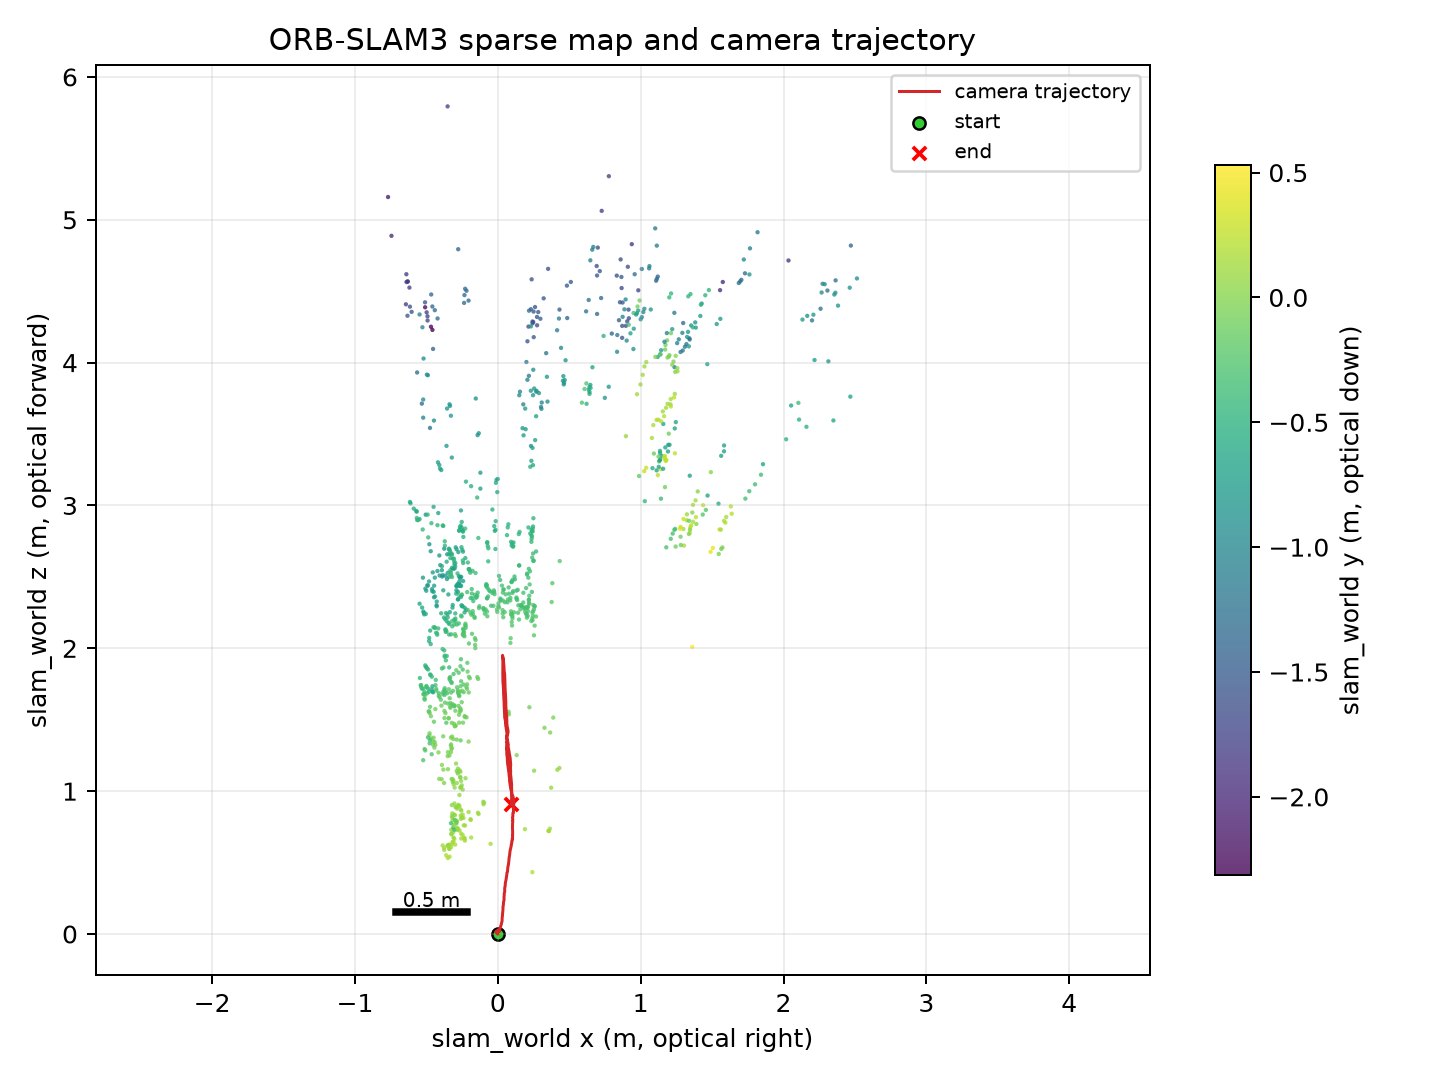
\includegraphics[width=0.9\textwidth]{figures/orbslam3-topdown.png}\caption{Quỹ đạo và map thưa, đoạn 2 m; bộ bằng chứng lab ngày 25/10.}\end{figure}
\begin{figure}[H]\centering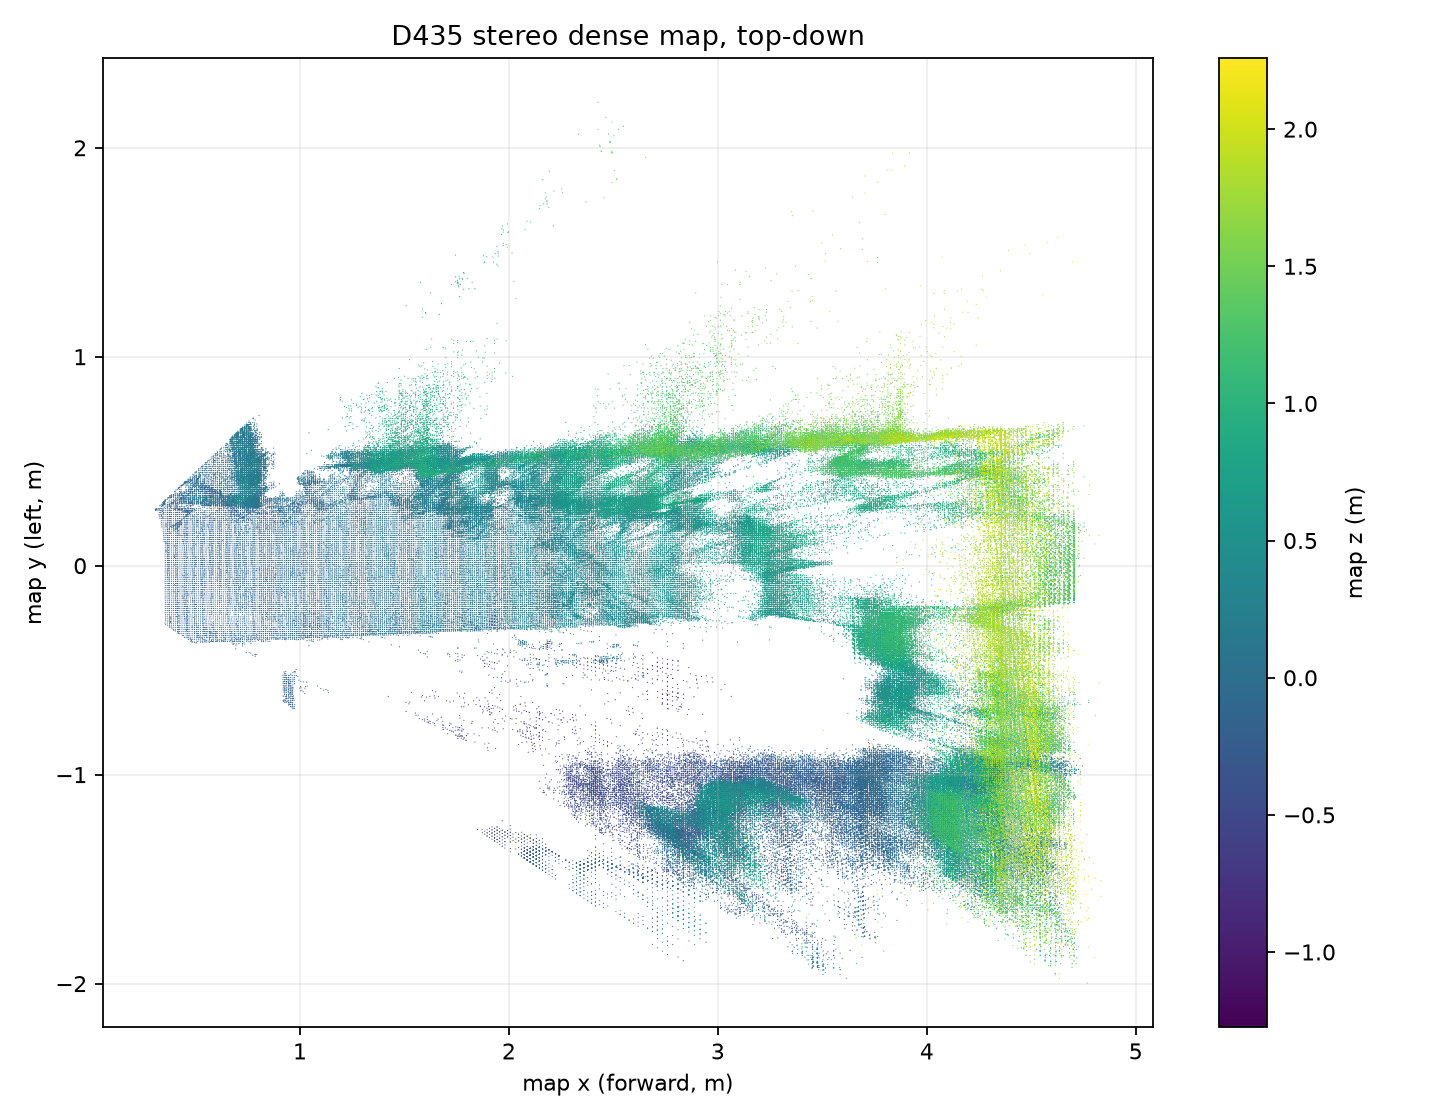
\includegraphics[width=0.9\textwidth]{figures/dense-map-topdown.png}\caption{Bản đồ dày đặc; bộ bằng chứng lab ngày 25/10.}\end{figure}
\begin{figure}[H]\centering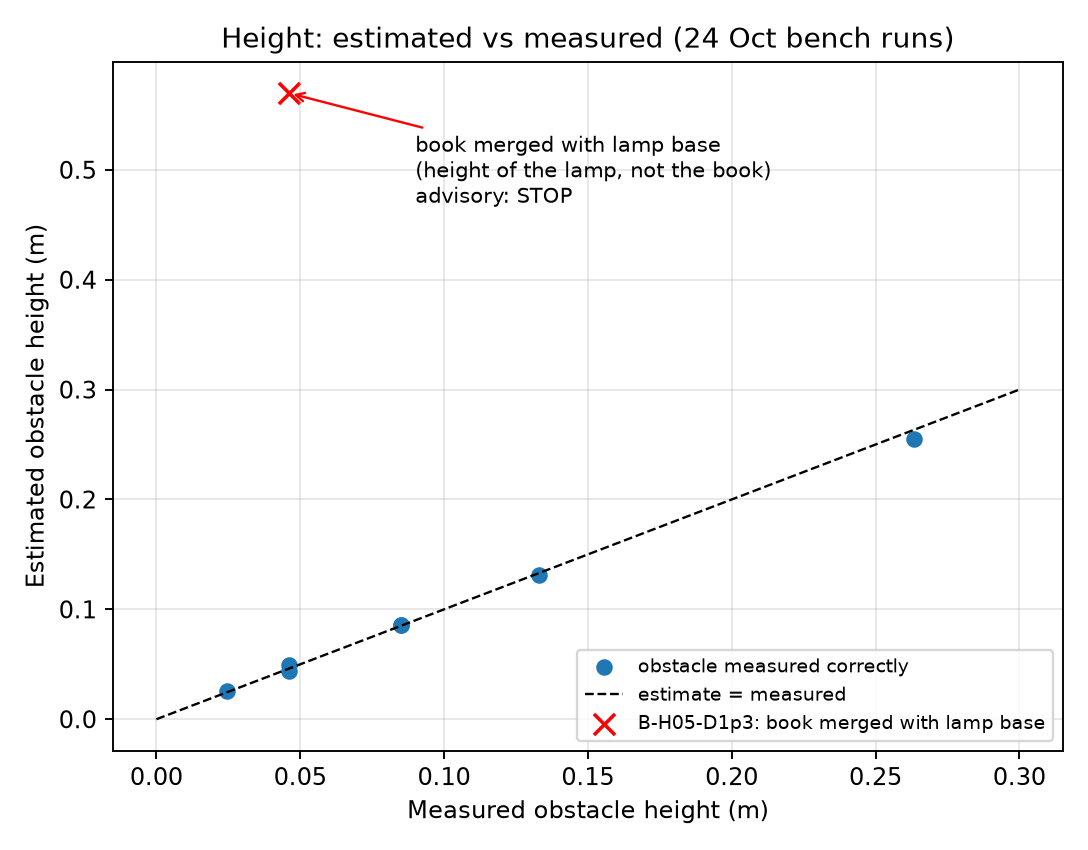
\includegraphics[width=0.9\textwidth]{figures/height-estimated-vs-measured.png}\caption{Chiều cao ước lượng so với đo, đánh giá bàn 24/10; các lượt đã được dùng khi chỉnh phương pháp.}\end{figure}
\begin{figure}[H]\centering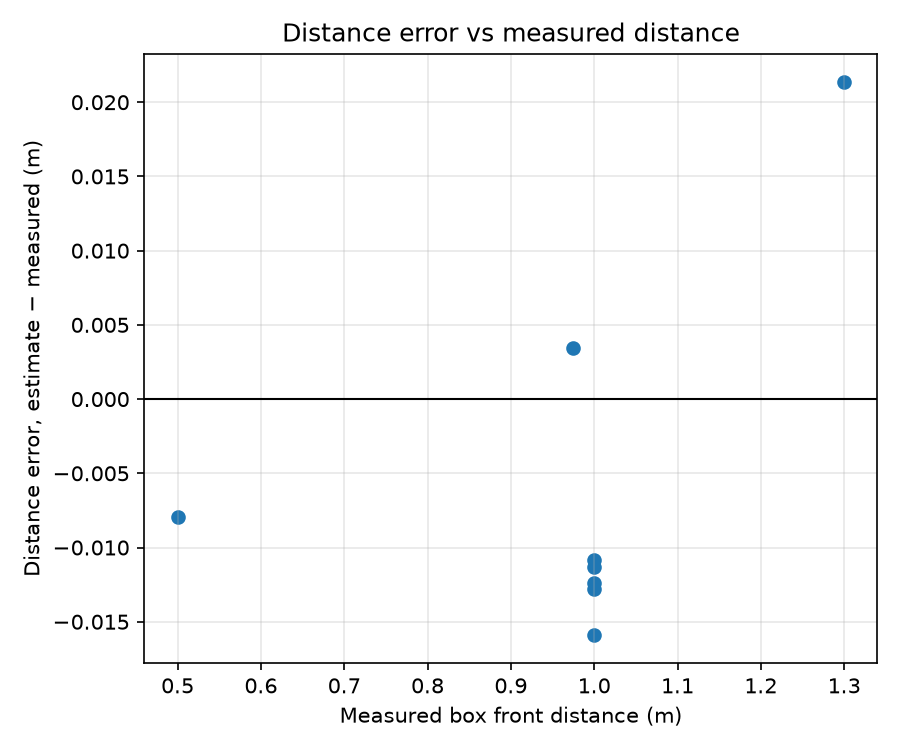
\includegraphics[width=0.9\textwidth]{figures/distance-error-vs-distance.png}\caption{Sai số khoảng cách theo cự ly, đánh giá bàn 24/10; không phải kiểm định độc lập.}\end{figure}

\section{Board minh hoạ F446RE}
Nucleo-F446RE thay vai trò giao diện STM32H7 để trình diễn micro-ROS và luồng \texttt{/cmd\_vel}; kiểm tra phần mềm ngày 26/10 xác nhận chuỗi đến topic \texttt{/cmd\_vel}. Demo nhận lại bản ghi camera, safety filter là chính sách minh hoạ; endpoint CAN tạo phản hồi motor giả. Không suy ra dừng xe thật hay đáp ứng RobStride. CAN loopback và IMU MPU6050 đang \pending{} do cần hàn header module.

\begin{tabularx}{\linewidth}{@{}X p{0.36\linewidth}@{}}\toprule
Hạng mục & Kết quả ghi nhận\\\midrule
CAN loopback / fake motor & \fbox{\parbox[c][0.48cm][c]{0.93\linewidth}{\centering\scriptsize Bổ sung sau khi hàn: kết quả CAN loopback}}\\
IMU MPU6050 & \fbox{\parbox[c][0.48cm][c]{0.93\linewidth}{\centering\scriptsize Bổ sung sau khi hàn: kết quả IMU}}\\
Đèn advisory & Đã thử trên board F446\\
Chuỗi demo đến \texttt{/cmd\_vel} & Đã xác minh phần mềm 26/10\\\bottomrule\end{tabularx}

\photo{1.15cm}{board F446 nhìn từ trên xuống, thấy rõ Nucleo, module CAN, dây nối và LED đỏ/xanh đang sáng; chụp sau khi hàn header và chạy thử.}

\section{Firmware STM32H7 và giám sát CAN}
Firmware AGV H7 đã thêm subscriber \texttt{/terrain\_advisory}, vùng đệm tĩnh 8 số thực, kiểm tra dữ liệu, bộ đếm hợp lệ/từ chối, tuổi dữ liệu 300 ms và hiển thị LCD; callback không gọi đường điều khiển motor. Tăng executor từ 4 lên 5 handle. Bản build đo được: text 207,184 B, data 14,880 B, bss 273,864 B. Đường xử lý lệnh và motor giữ nguyên. \pending{} xác minh nạp/chạy trên bo H7 mới. Monitor CAN hai bus ở chế độ listen-only đã sẵn sàng bằng firmware F446; chưa ghi nhận bus vật lý.

\section{Video demo}
\begin{minipage}{\linewidth}\centering\fbox{\parbox[c][0.72cm][c]{0.94\linewidth}{\centering\small [LIÊN KẾT / QR VIDEO: chủ dự án bổ sung sau khi quay]}}\end{minipage}
\textbf{Kịch bản quay 60--90 giây:} (1) toàn cảnh rig D435i và board; (2) Foxglove phát lại video và topic advisory; (3) hộp xuất hiện, STOP và LED đỏ; (4) vùng không vật cản, NONE và LED xanh; (5) màn hình \texttt{/cmd\_vel}, trạng thái safety filter, fake wheel feedback/IMU; (6) cận cảnh board và nhắc rõ đây là phát lại dữ liệu, CAN motor giả. Quay đôi: điện thoại quay LED đồng thời ghi màn hình Foxglove, sau đó ghép chia đôi màn hình; giữ máy ổn định, thêm chú thích, không cắt ghép để hàm ý cảm biến hoặc motor thật.

\photo{0.9cm}{ảnh chụp màn hình Foxglove trong demo: camera replay, terrain advisory, safety-filter state và fake wheel feedback cùng xuất hiện.}

\section{Kế hoạch tiếp theo}
\begin{itemize}\setlength{\itemsep}{0pt}
\item [\textbf{[ngày]}] Hàn header module; xác minh CAN loopback và đọc IMU trên F446, lưu log / ảnh.
\item [\textbf{[ngày]}] Cùng người phụ trách board chọn bo đích (H7 AGV hay WBR); thử subscriber chỉ hiển thị, motor disable, xác nhận stale/invalid.
\item [\textbf{[ngày]}] Chạy camera live qua Pi tới board; đo sequence, latency, mất gói và stale sau rút link.
\item [\textbf{[ngày]}] Chạy đồng thời ORB-SLAM3 + detector trên Pi; đo FPS, CPU, nhiệt độ, rớt khung và latency advisory.
\item [\textbf{[ngày]}] Chỉ sau khi duyệt gate và quy trình an toàn: thử trên giá đỡ / dây giữ; chưa cấp quyền nhảy từ Pi.
\end{itemize}
\section{Hạn chế hiện tại}
\begin{itemize}\setlength{\itemsep}{0pt}
\item ORB-SLAM3 và detector chưa chạy đồng thời trên camera live; chưa có số tải Pi trong chế độ kết hợp.
\item Lượt ORB 2 m bị cắt trước lượt quay về; EuRoC là kết quả offline, lệch frame/extrinsic còn là giả thiết trong phép so sánh.
\item Hysteresis giảm flicker khi replay nhưng flicker LED live còn cao ở mép ngưỡng; chưa chứng minh cải thiện ngoài rig.
\item CAN, IMU trên F446 và firmware H7 chưa được kiểm chứng vật lý; demo dùng camera replay và motor giả.
\item Ngưỡng phân loại và khoảng cách nhảy chưa được xác nhận trên WBR; chưa có thử nghiệm robot thật hoặc đánh giá an toàn chức năng.
\end{itemize}
\section*{Thuật ngữ nhanh}
\fbox{\begin{minipage}{0.97\textwidth}\small
\textbf{SLAM:} định vị và dựng bản đồ đồng thời từ cảm biến. \quad
\textbf{Keyframe:} khung hình đại diện được chọn để cập nhật bản đồ.\\
\textbf{ATE:} sai số quỹ đạo tuyệt đối sau khi căn chỉnh quỹ đạo ước lượng với tham chiếu. \quad
\textbf{micro-ROS:} lớp ROS 2 gọn cho vi điều khiển.\\
\textbf{CAN:} mạng truyền thông bus dùng phổ biến giữa bộ điều khiển và thiết bị. \quad
\textbf{Advisory:} thông tin khuyến nghị/trạng thái cho bộ điều khiển hoặc người vận hành; không trực tiếp cấp quyền chấp hành motor.
\end{minipage}}
\vfill\scriptsize Nguồn nội bộ: báo cáo lab 25/10; đánh giá detector và UART 24/10; giao diện advisory; ghi chú build H7; kịch bản demo F446. Số liệu đo và phạm vi thử được ghi cạnh từng kết quả.
\end{document}
